

\subsection{WebSocket based GUI Application}

 	\begin{figure}[H]
    		\centering
    		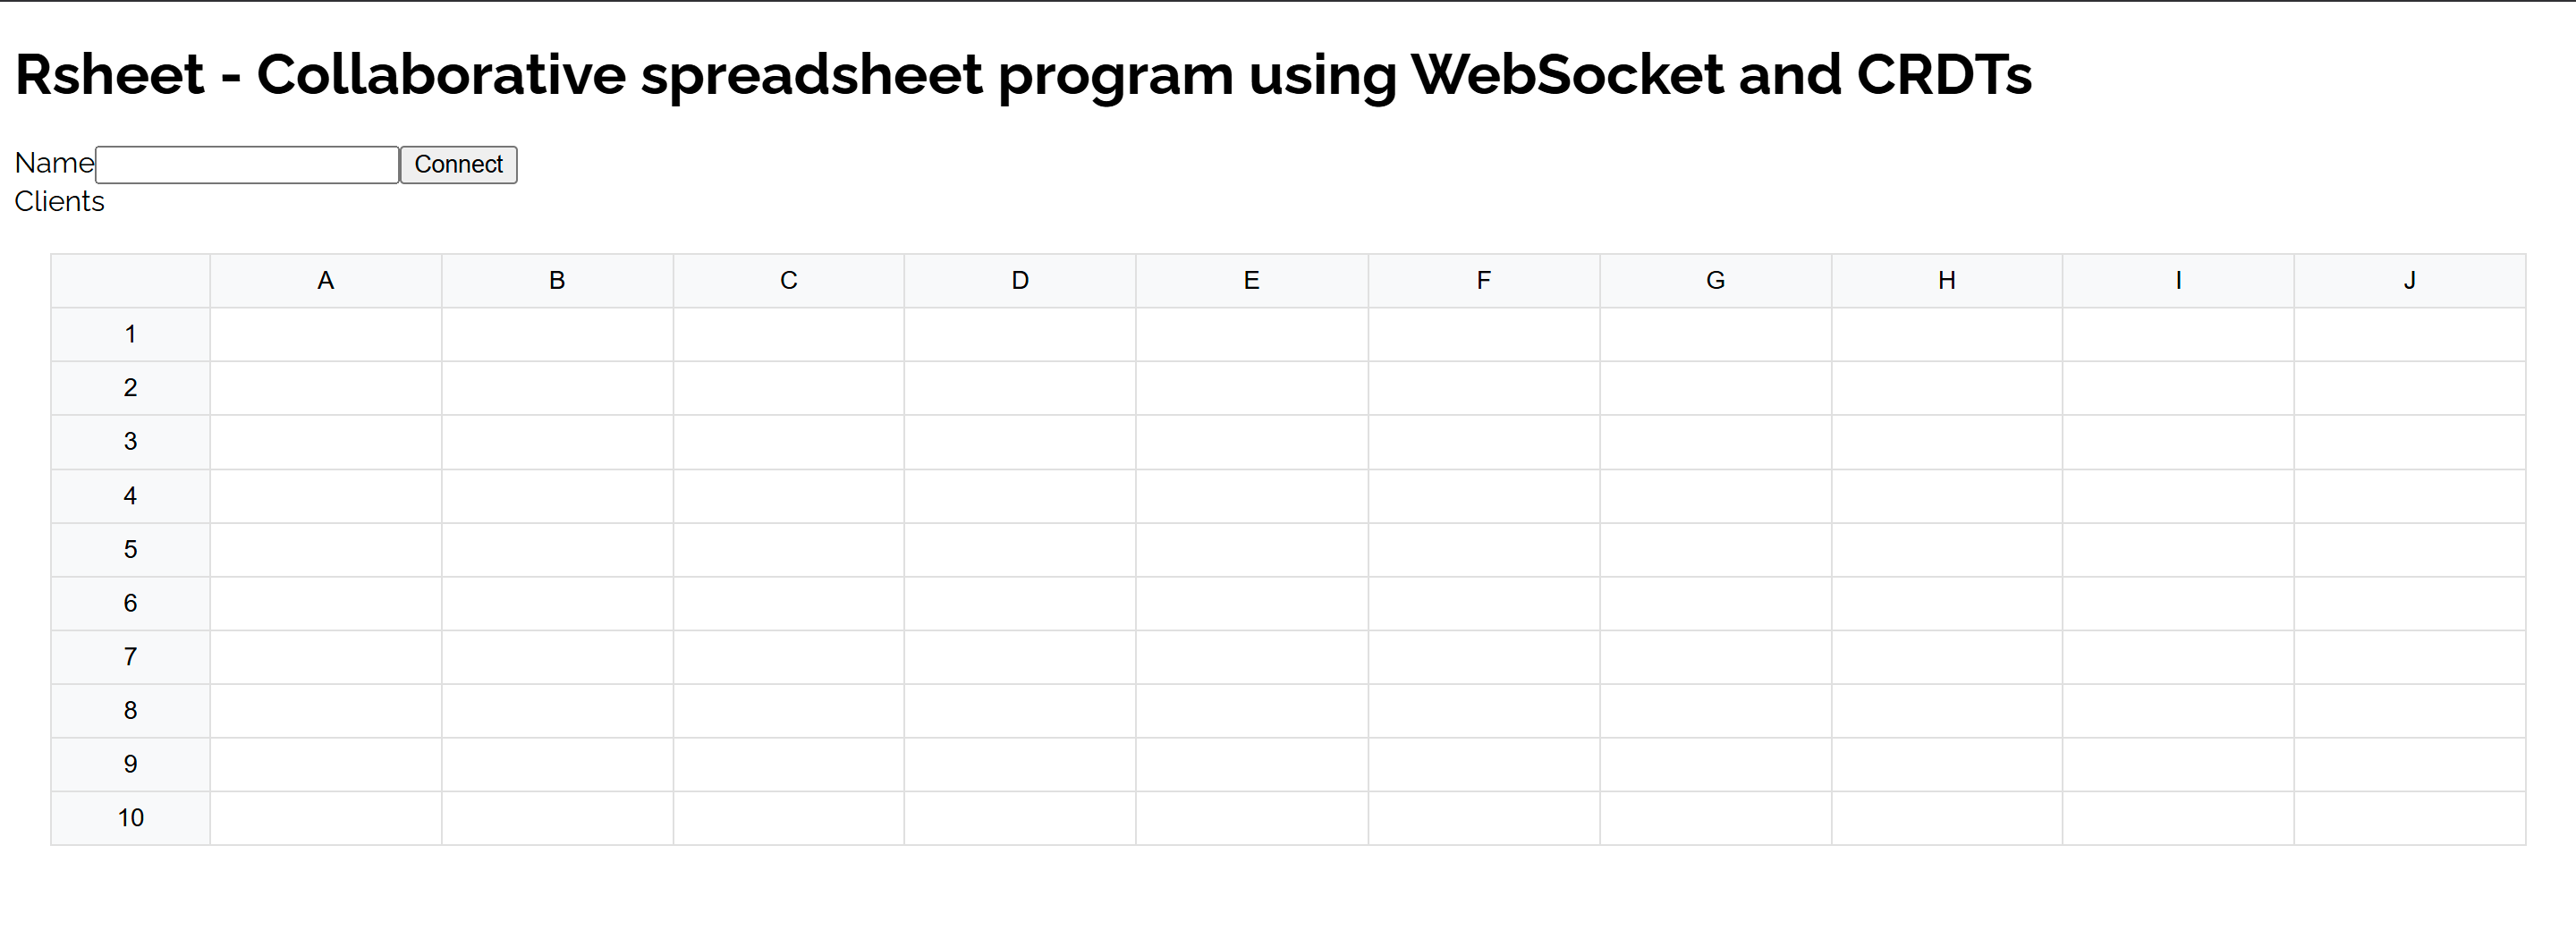
\includegraphics[width=0.75\columnwidth]{figures/crdt1.png}
    		\caption{Frontend of the CRDT-enabled websocket application.}
    		\label{fig:figure}
    	\end{figure}

 	\begin{figure}[H]
    		\centering
    		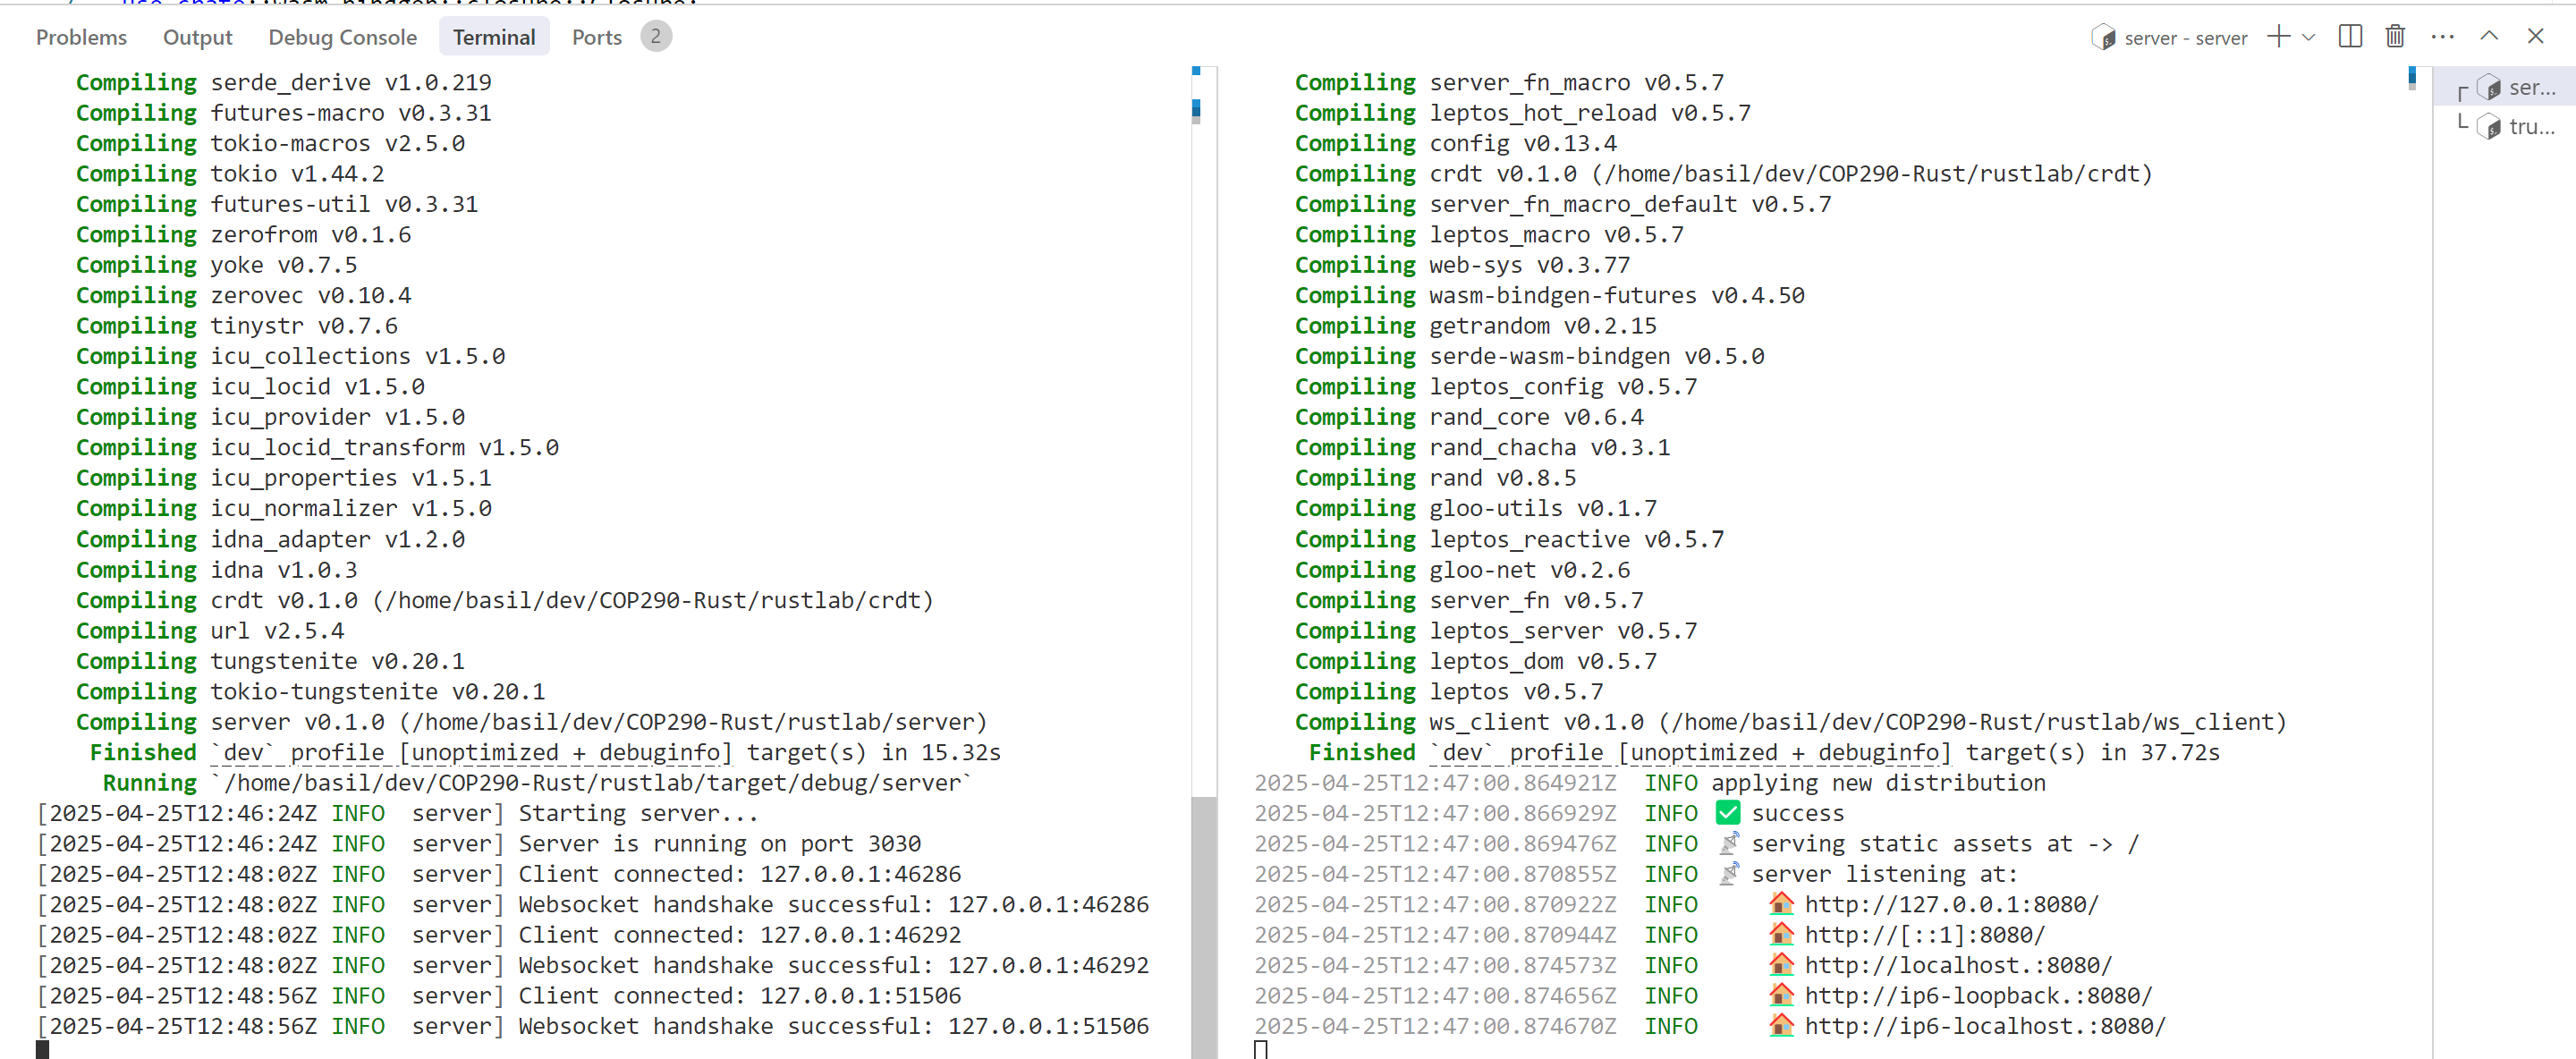
\includegraphics[width=0.75\columnwidth]{figures/crdt2.png}
    		\caption{Screenshot of the terminal showing server and client processes.}
    		\label{fig:figure}
    	\end{figure}

        \begin{figure}[H]
    		\centering
    		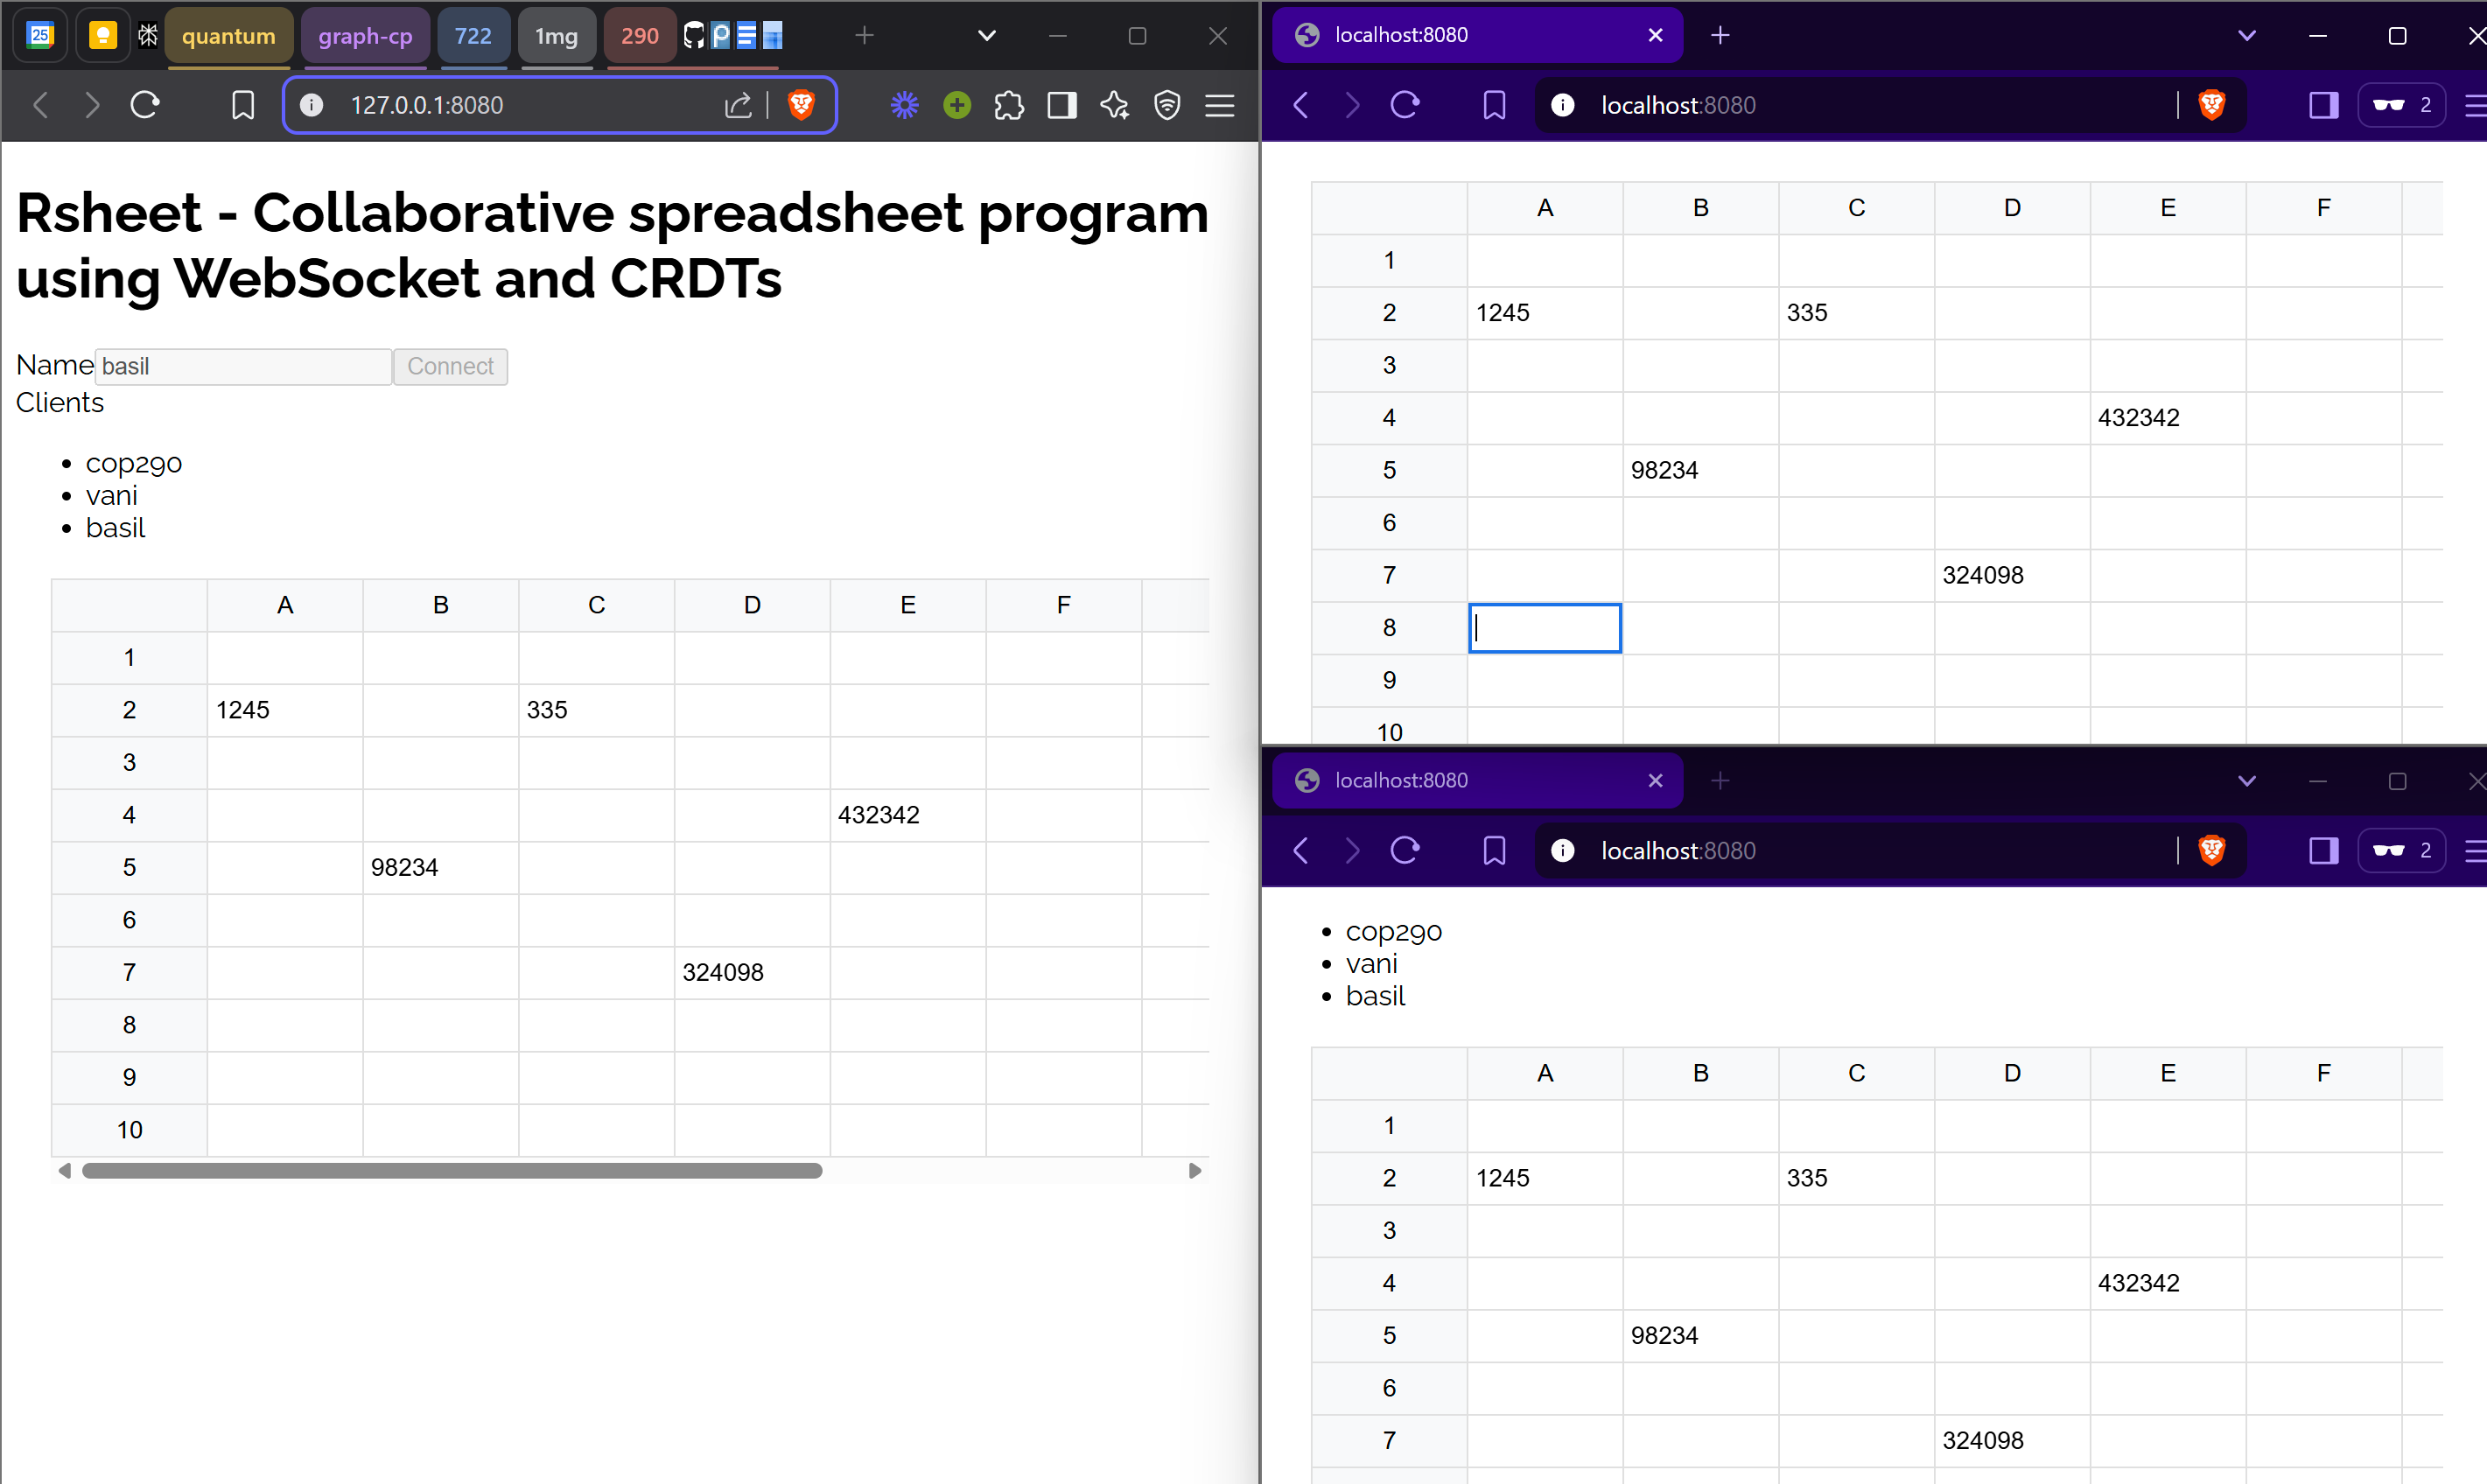
\includegraphics[width=0.75\columnwidth]{figures/crdt3.png}
    		\caption{Screenshot showing multiple users interacting with the same spreadsheet.}
    		\label{fig:figure}
    	\end{figure}

\subsection{Client-Server based GUI Application}

 	\begin{figure}[H]
    		\centering
    		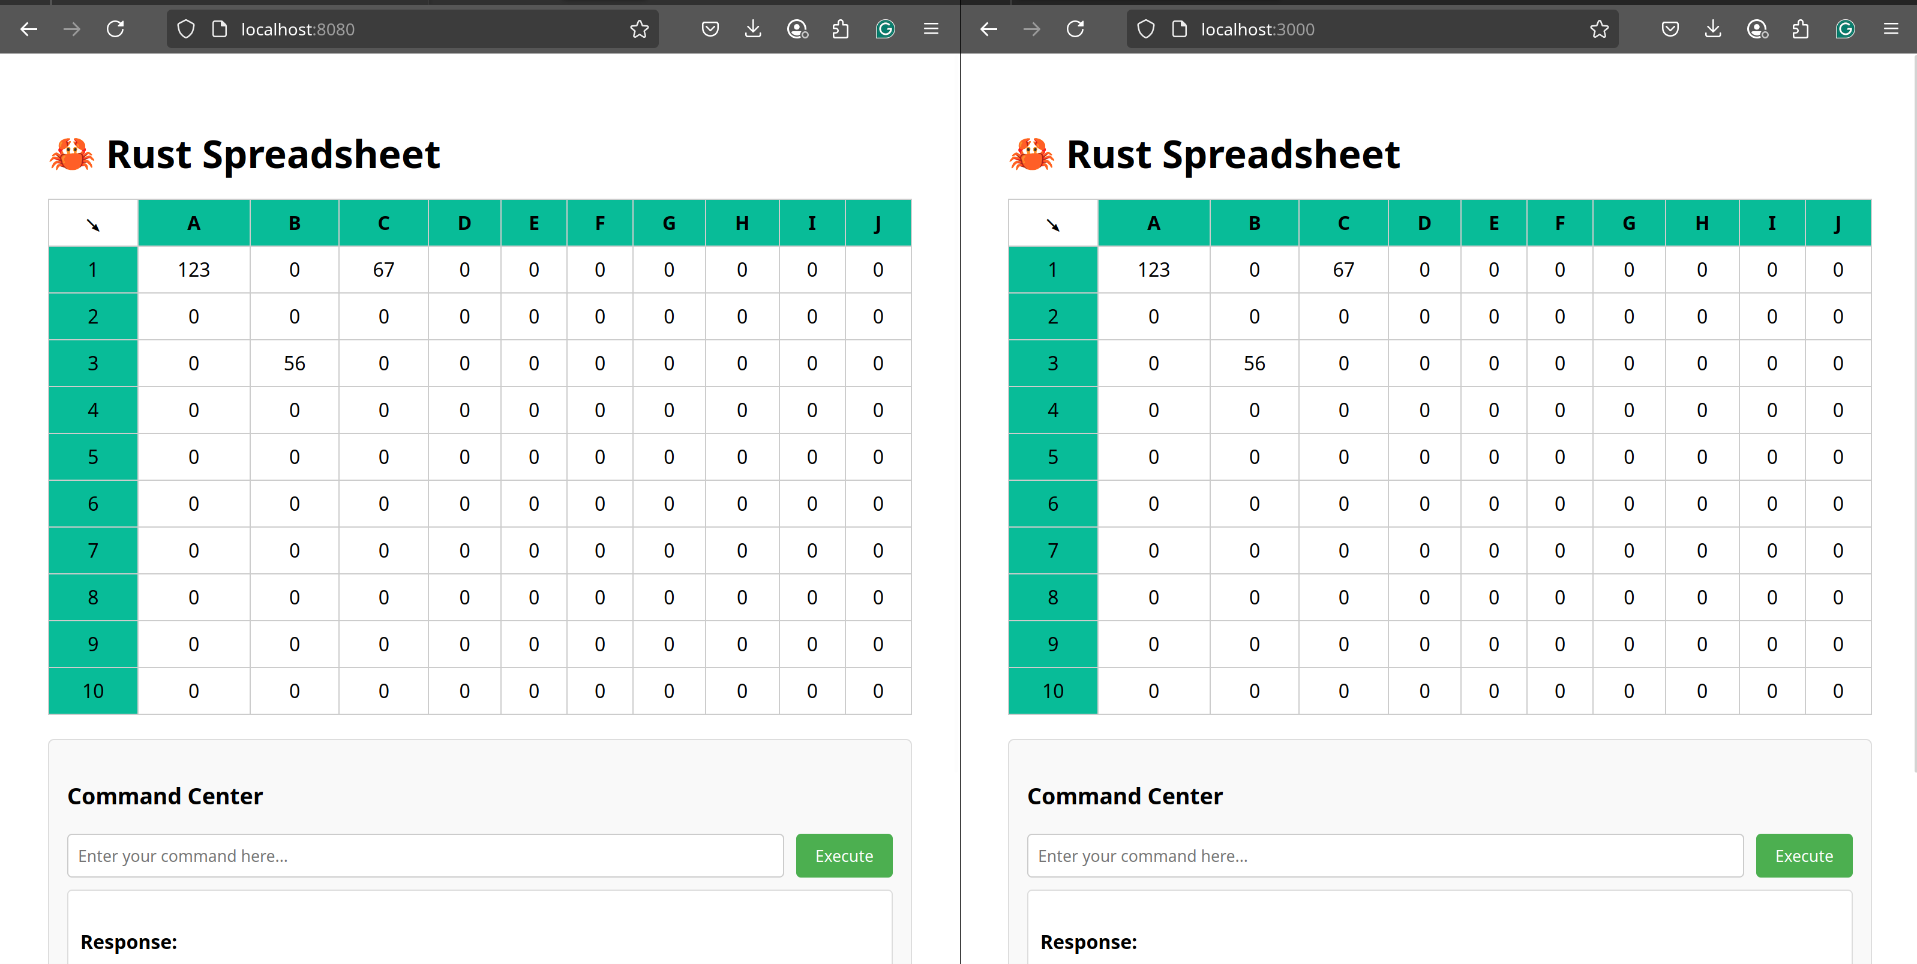
\includegraphics[width=0.75\columnwidth]{figures/2_servers_gui.png}
    		\caption{Screenshot of multiple clients.}
    		\label{fig:figure}
    	\end{figure}

        \begin{figure}[H]
            \centering
            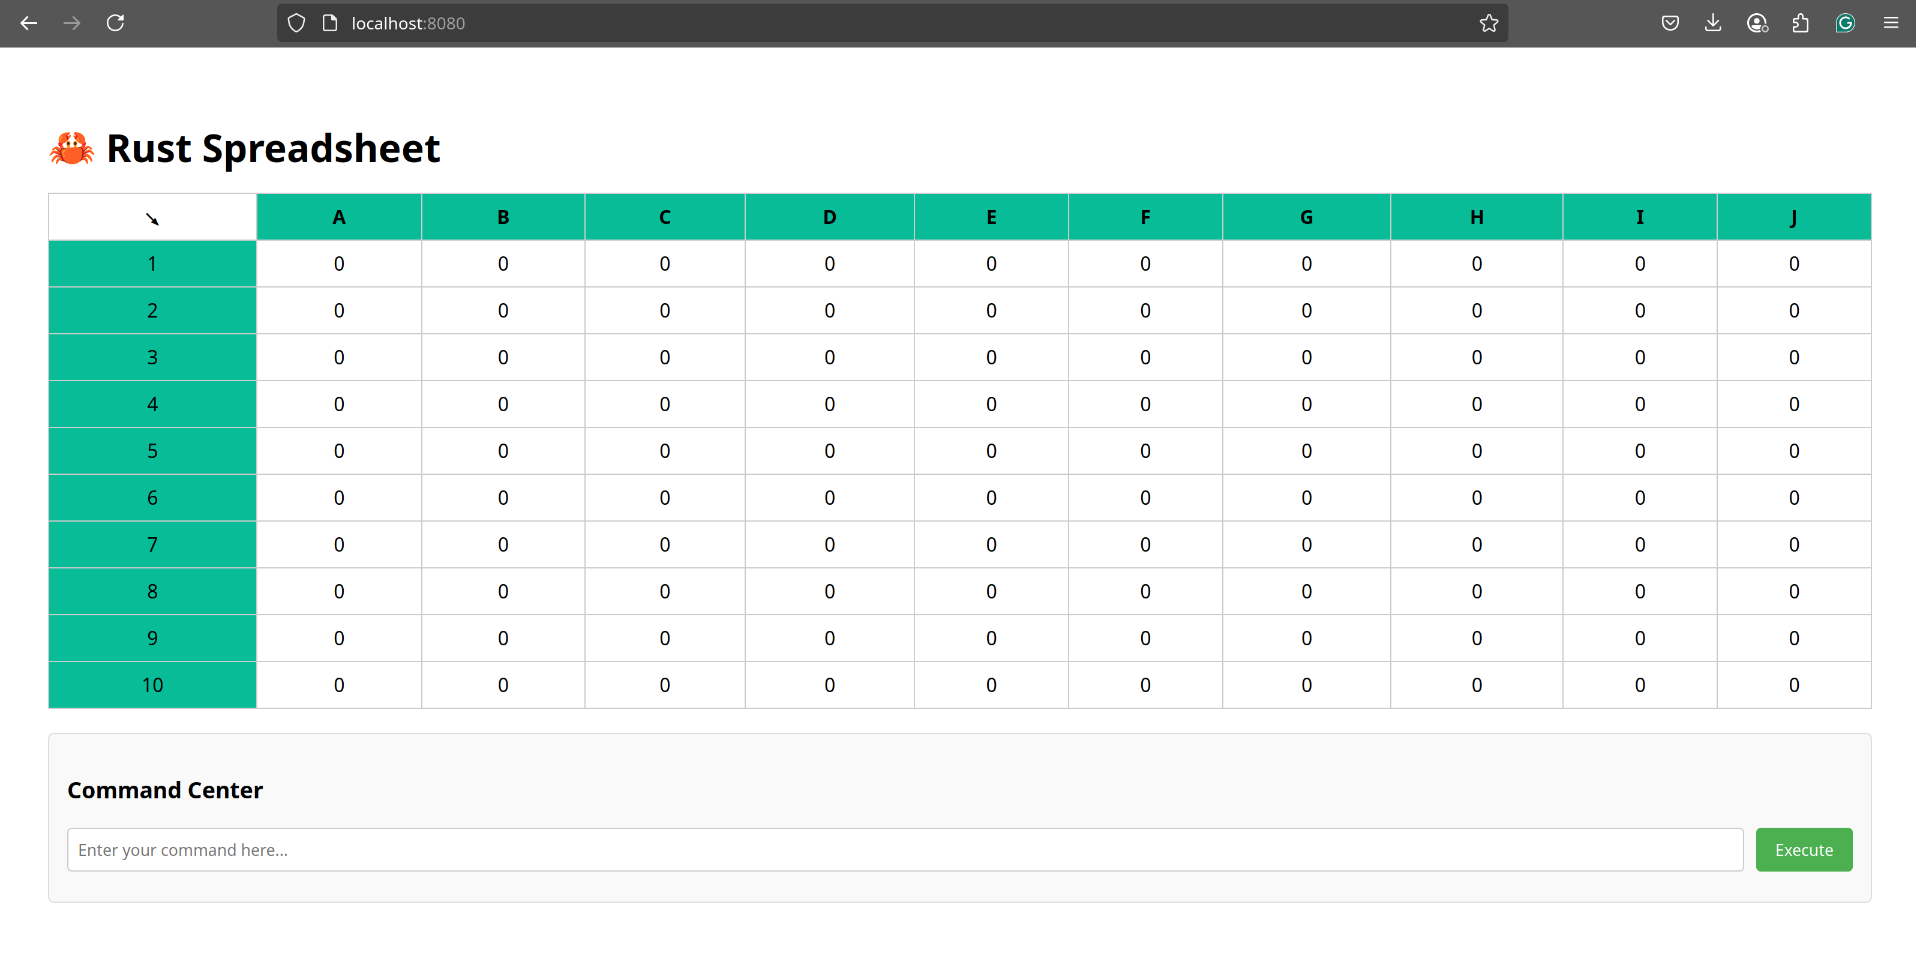
\includegraphics[width=0.75\linewidth]{figures/Web_GUI.png}
            \caption{Showcasing Web GUI}
            \label{fig:enter-label}
        \end{figure}

        \begin{figure}[H]
            \centering
            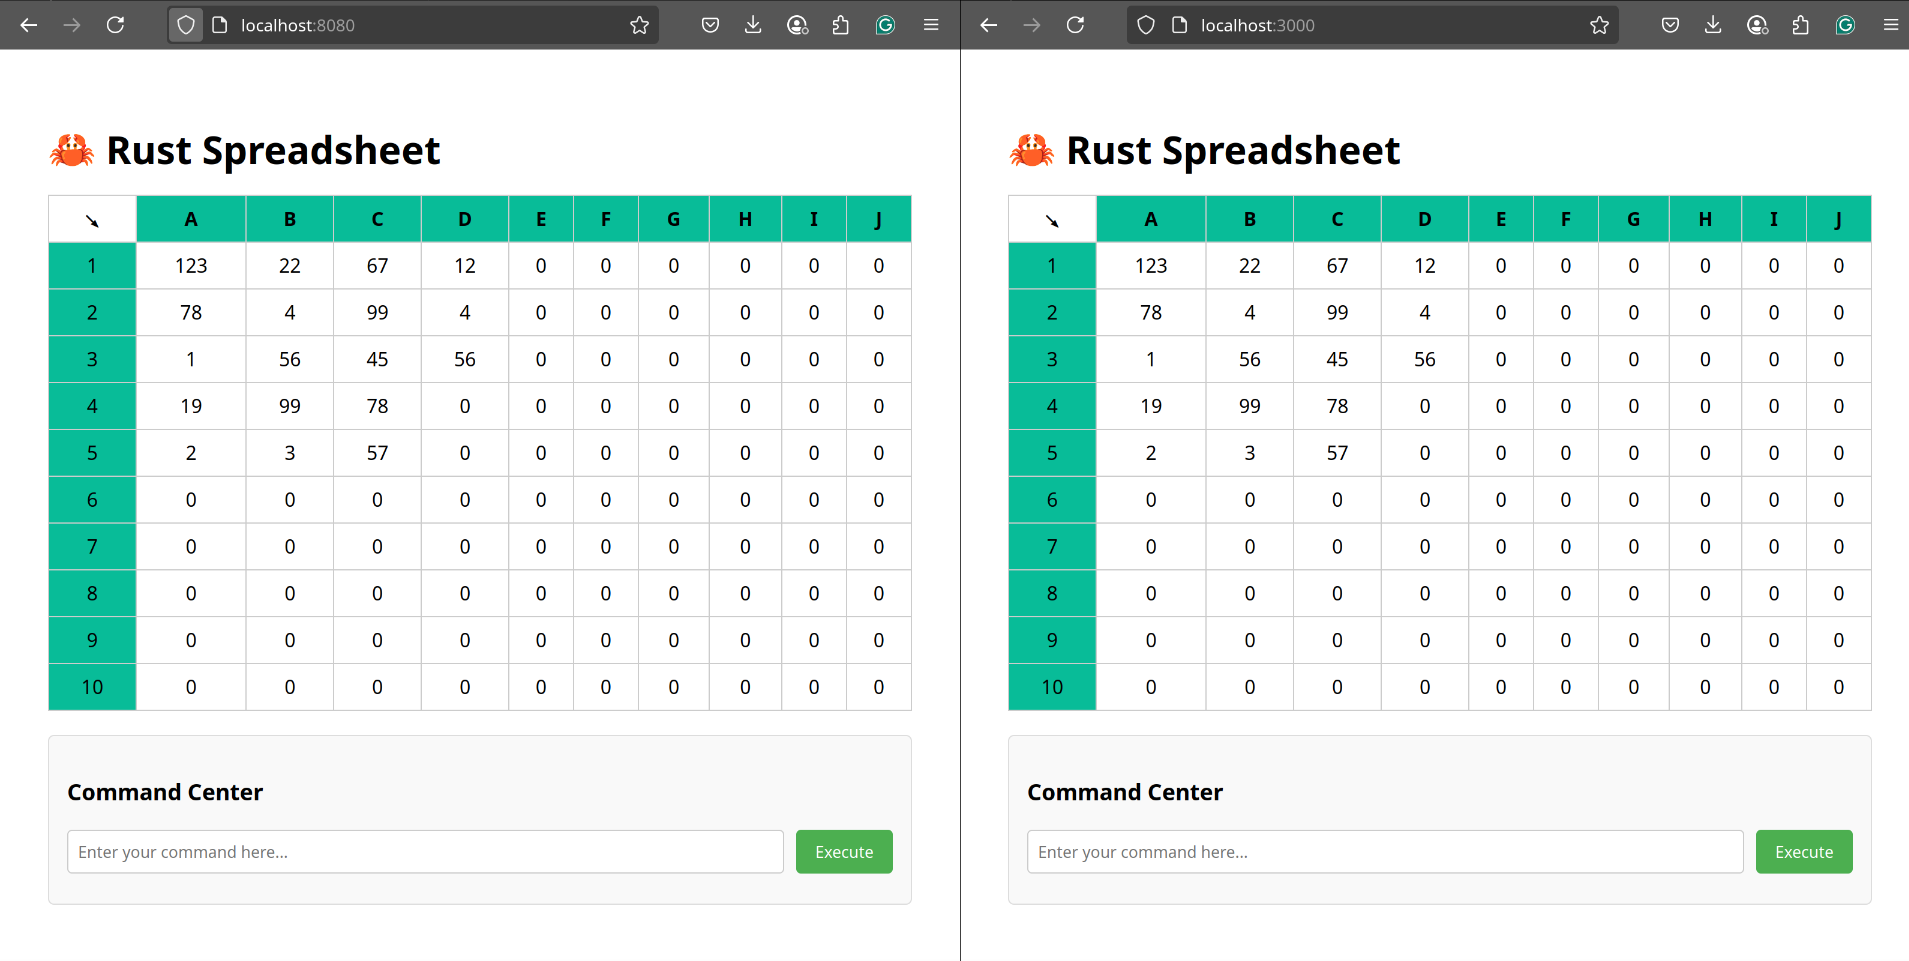
\includegraphics[width=0.75\linewidth]{figures/sync_data_gui.png}
            \caption{Synchronizing data between different clients}
            \label{fig:enter-label}
        \end{figure}

\subsection{Extended TUI Application}

        \begin{figure}[H]
            \centering
            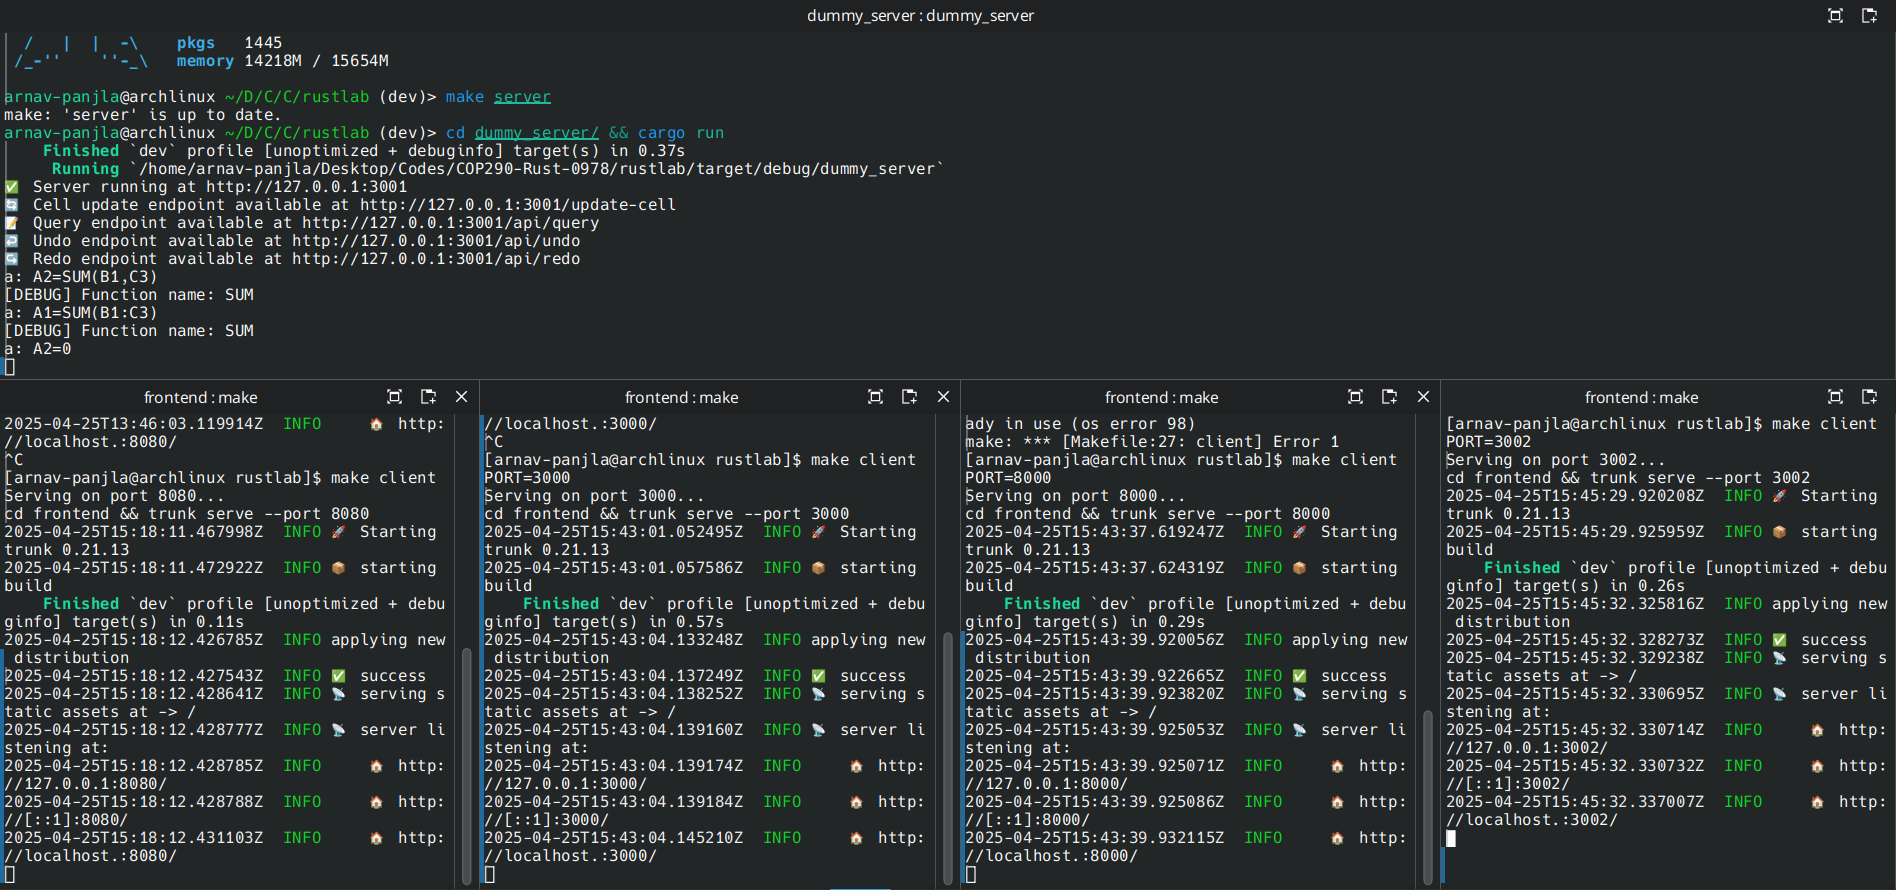
\includegraphics[width=0.75\linewidth]{figures/runnning_multiple_clients.png}
            \caption{Running multiple clients}
            \label{fig:enter-label}
        \end{figure}

        \begin{figure}[H]
            \centering
            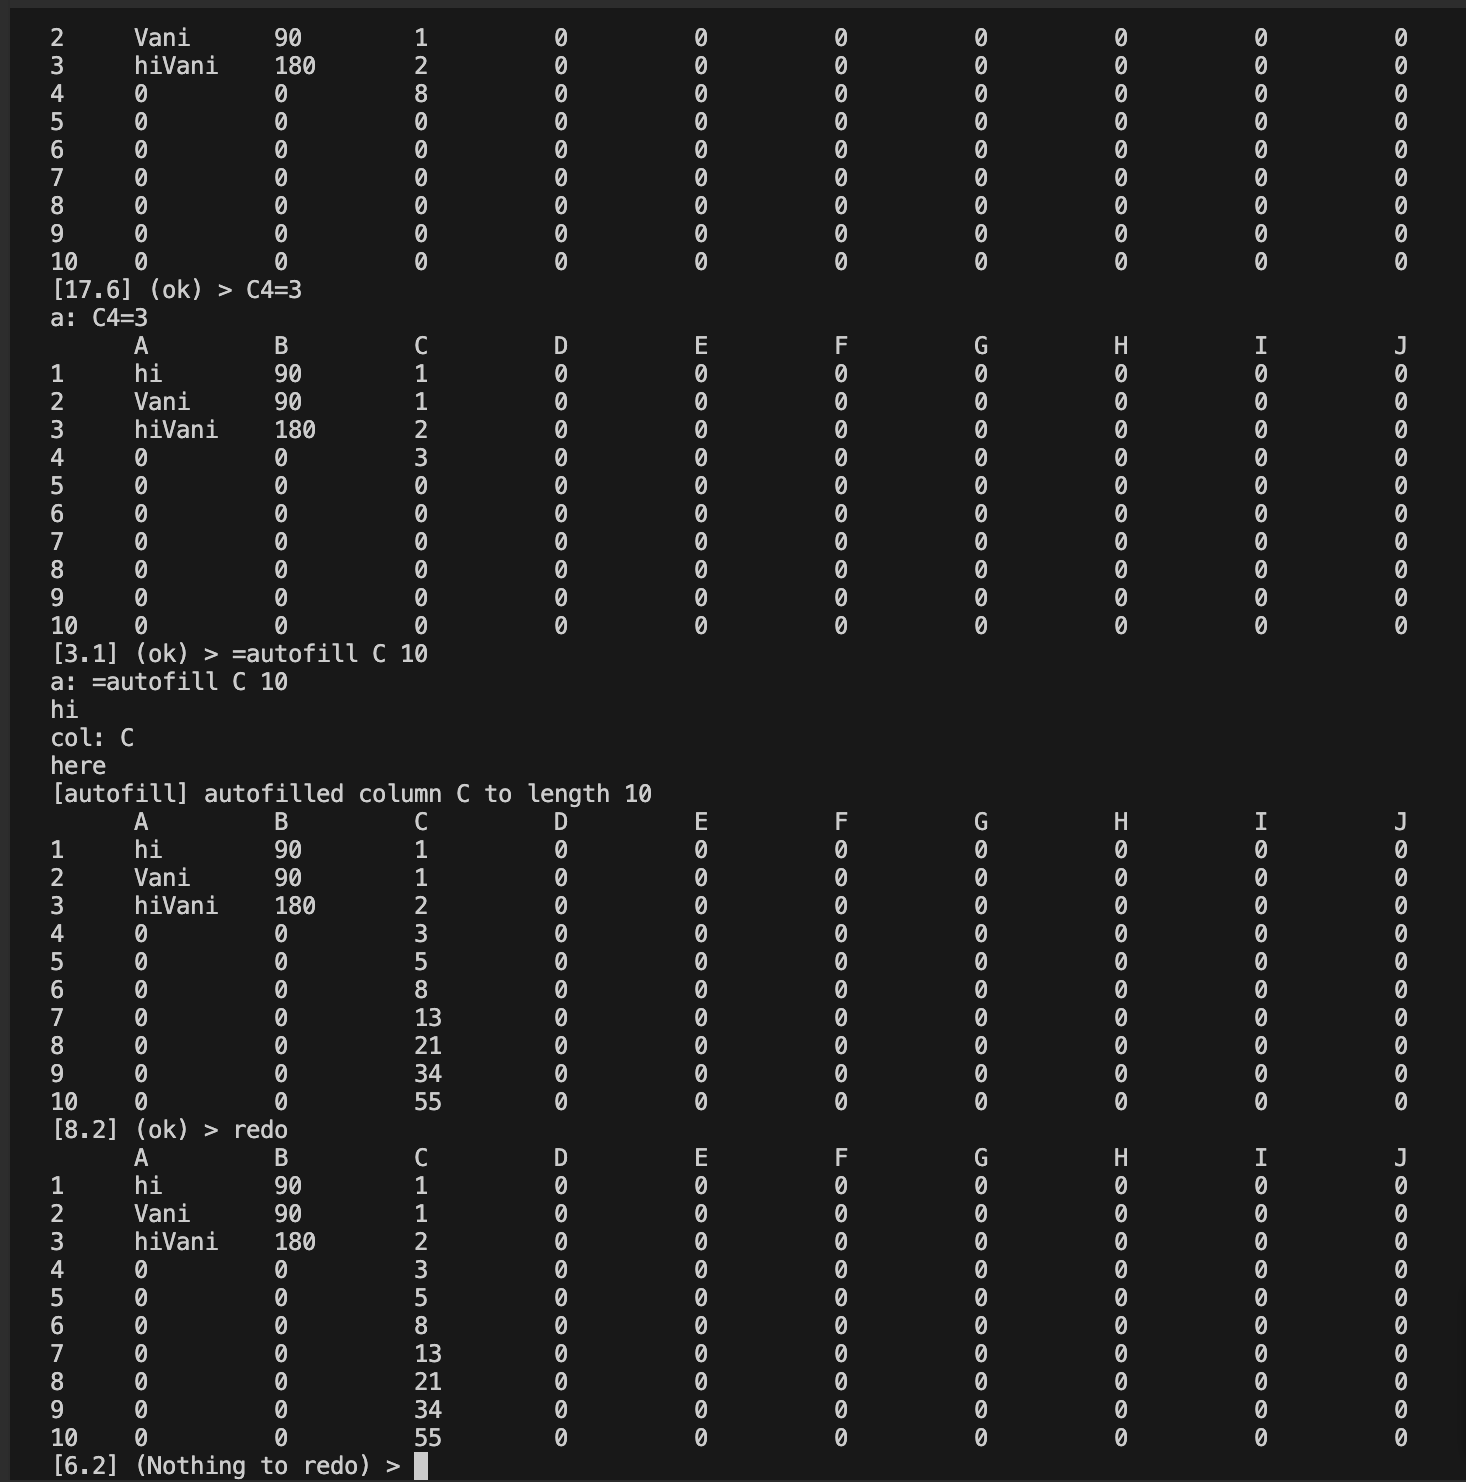
\includegraphics[width=0.5\linewidth]{image.png}
            \caption{Performing string concatenation}
            \label{fig:enter-label}
        \end{figure}

        \begin{figure}[H]
            \centering
            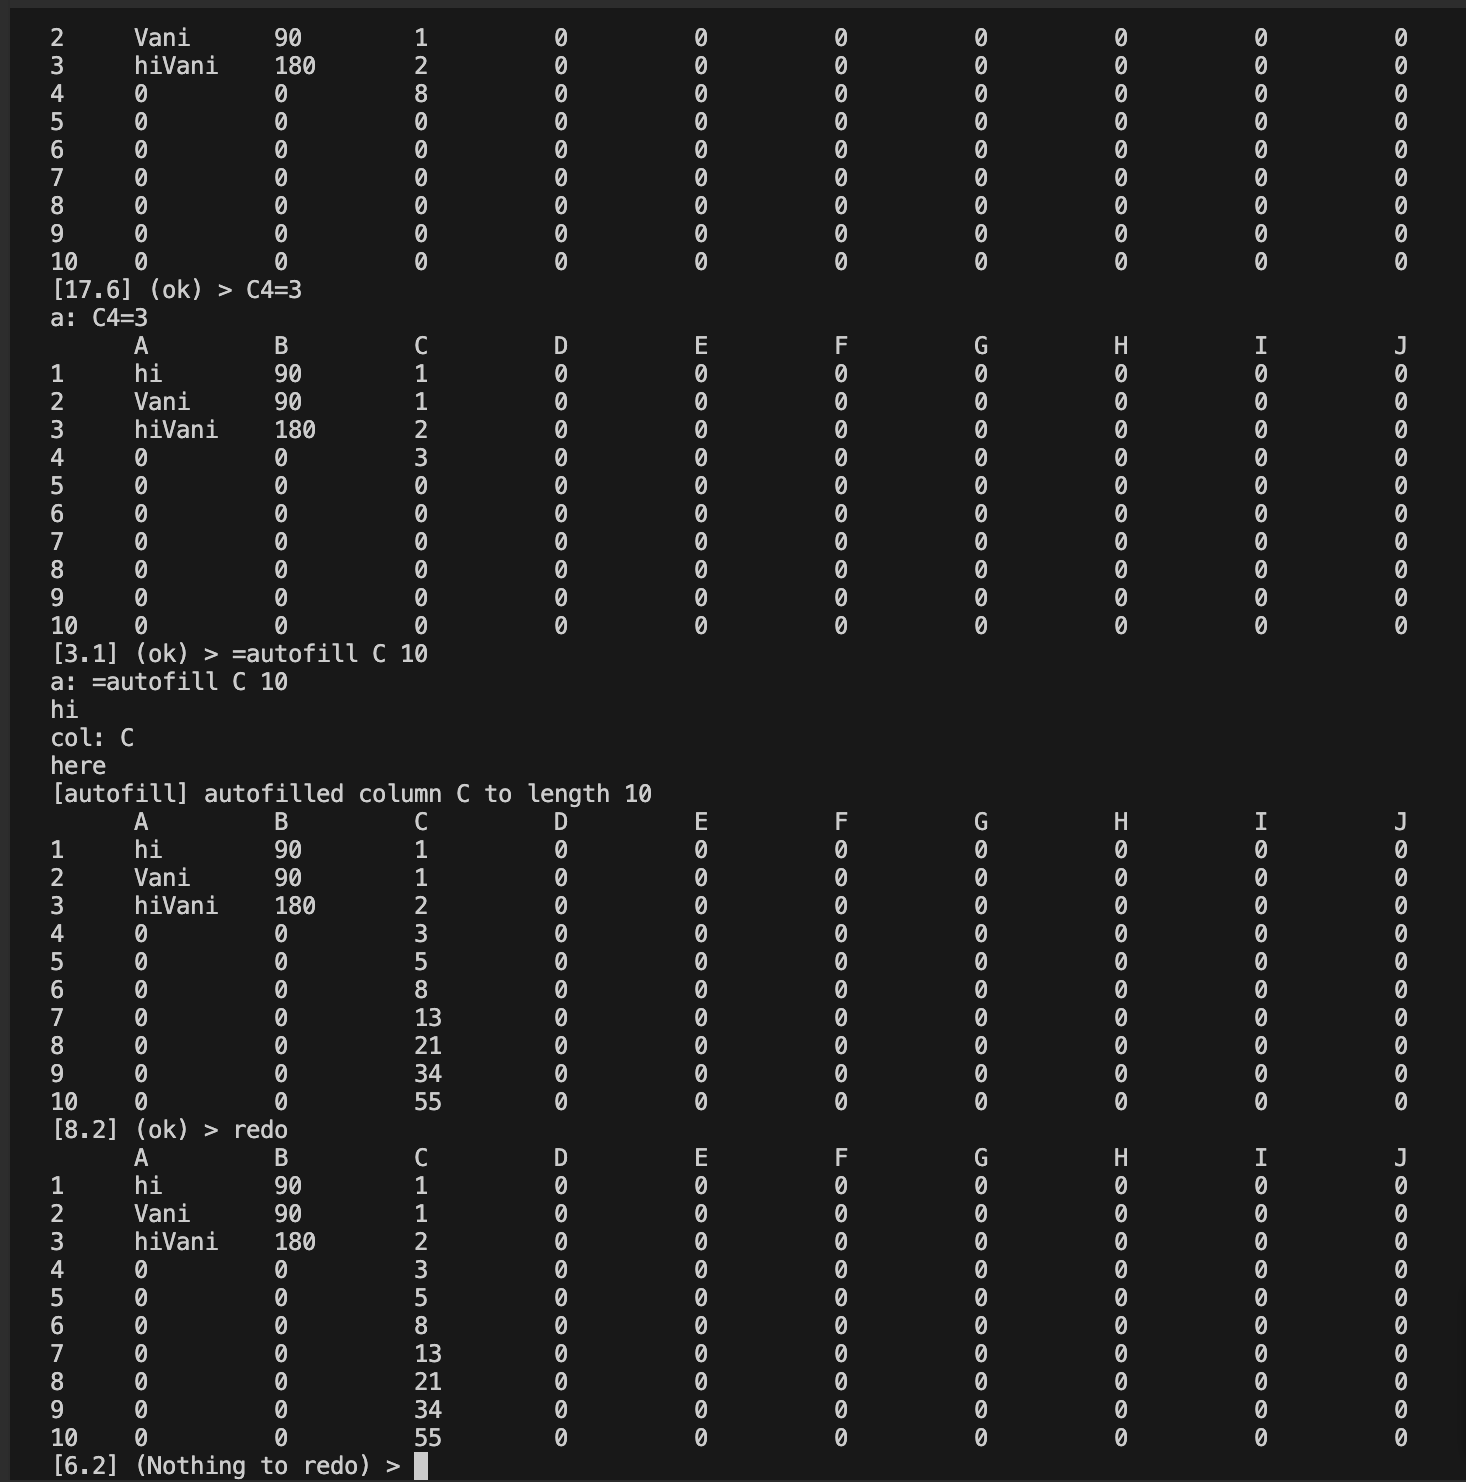
\includegraphics[width=0.5\linewidth]{image.png}
            \caption{Performing recalculation and float-int addition}
            \label{fig:enter-label}
        \end{figure}
        
        \begin{figure}[H]
            \centering
            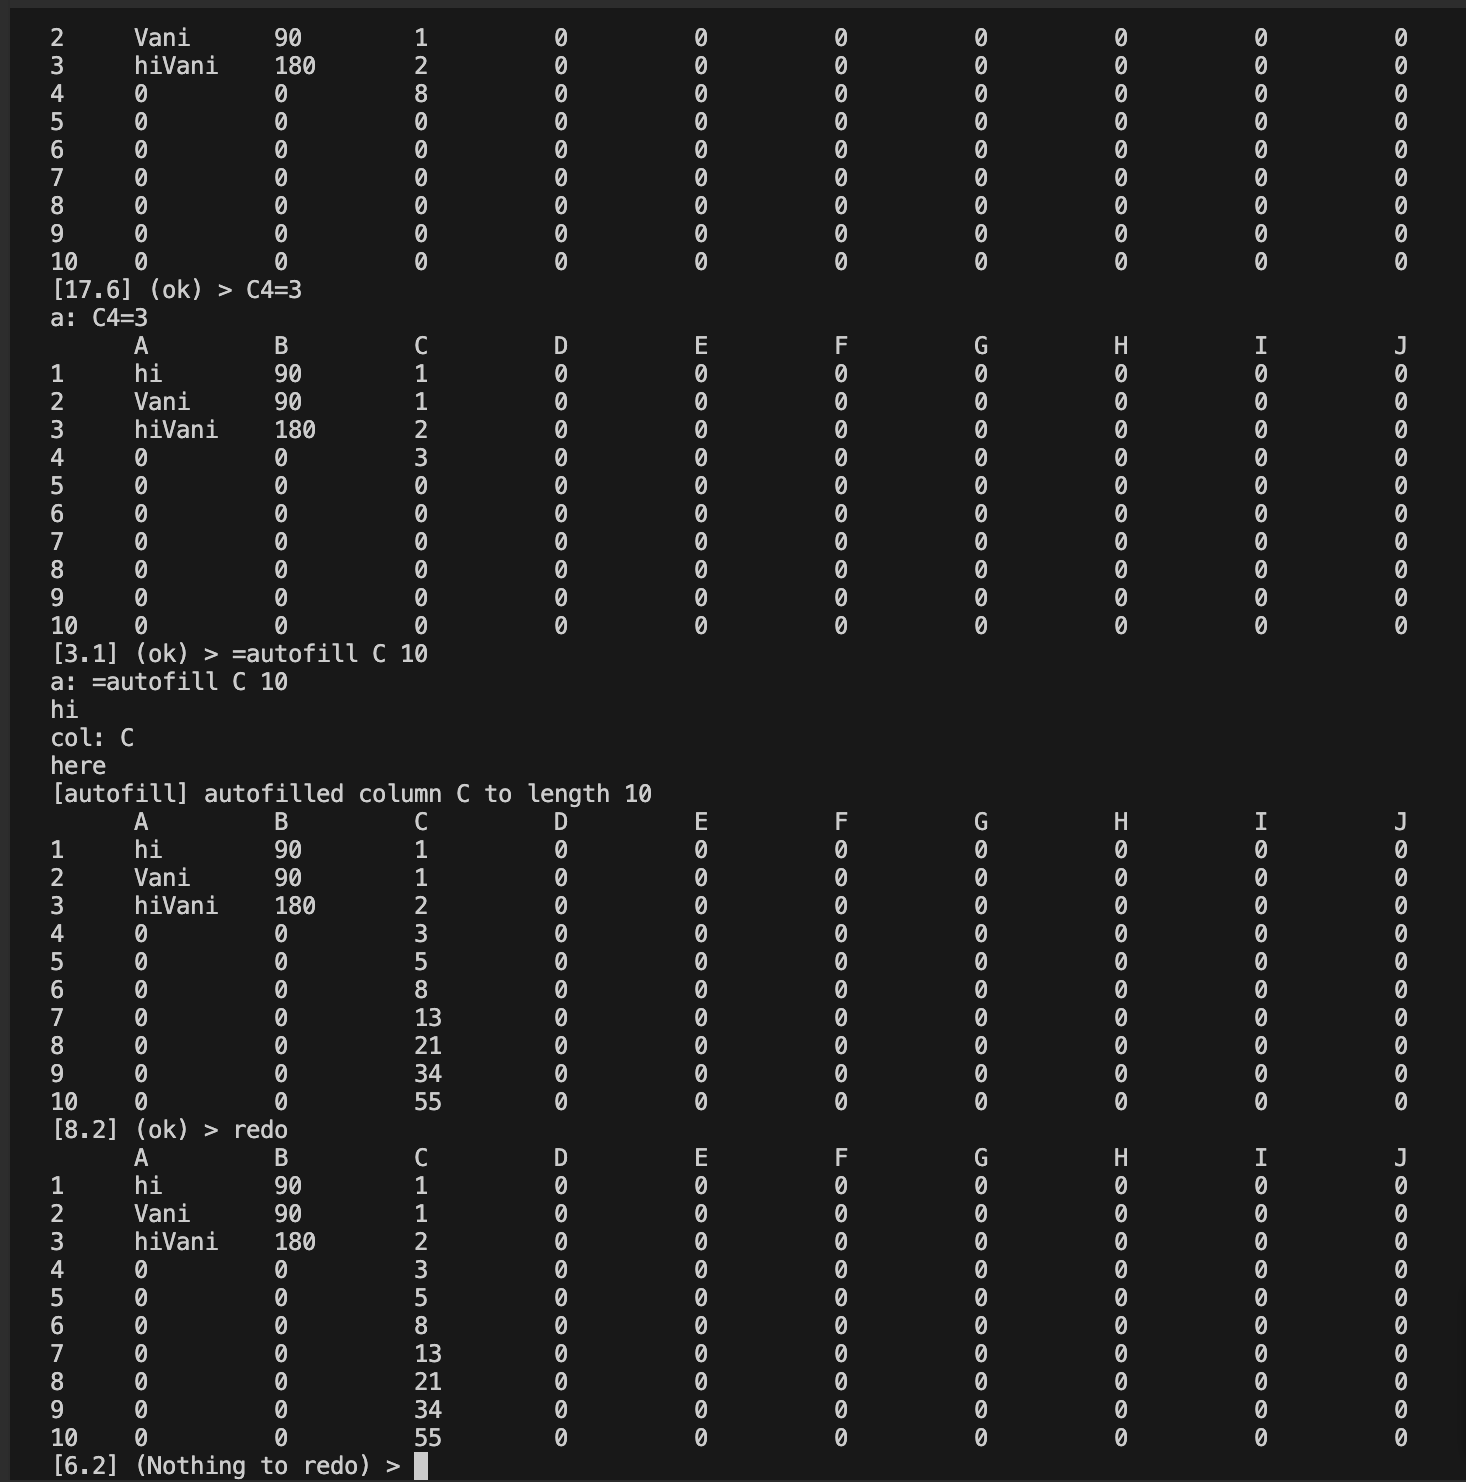
\includegraphics[width=0.5\linewidth]{image.png}
            \caption{Performing recalculation}
            \label{fig:enter-label}
        \end{figure}
        
        \begin{figure}[H]
            \centering
            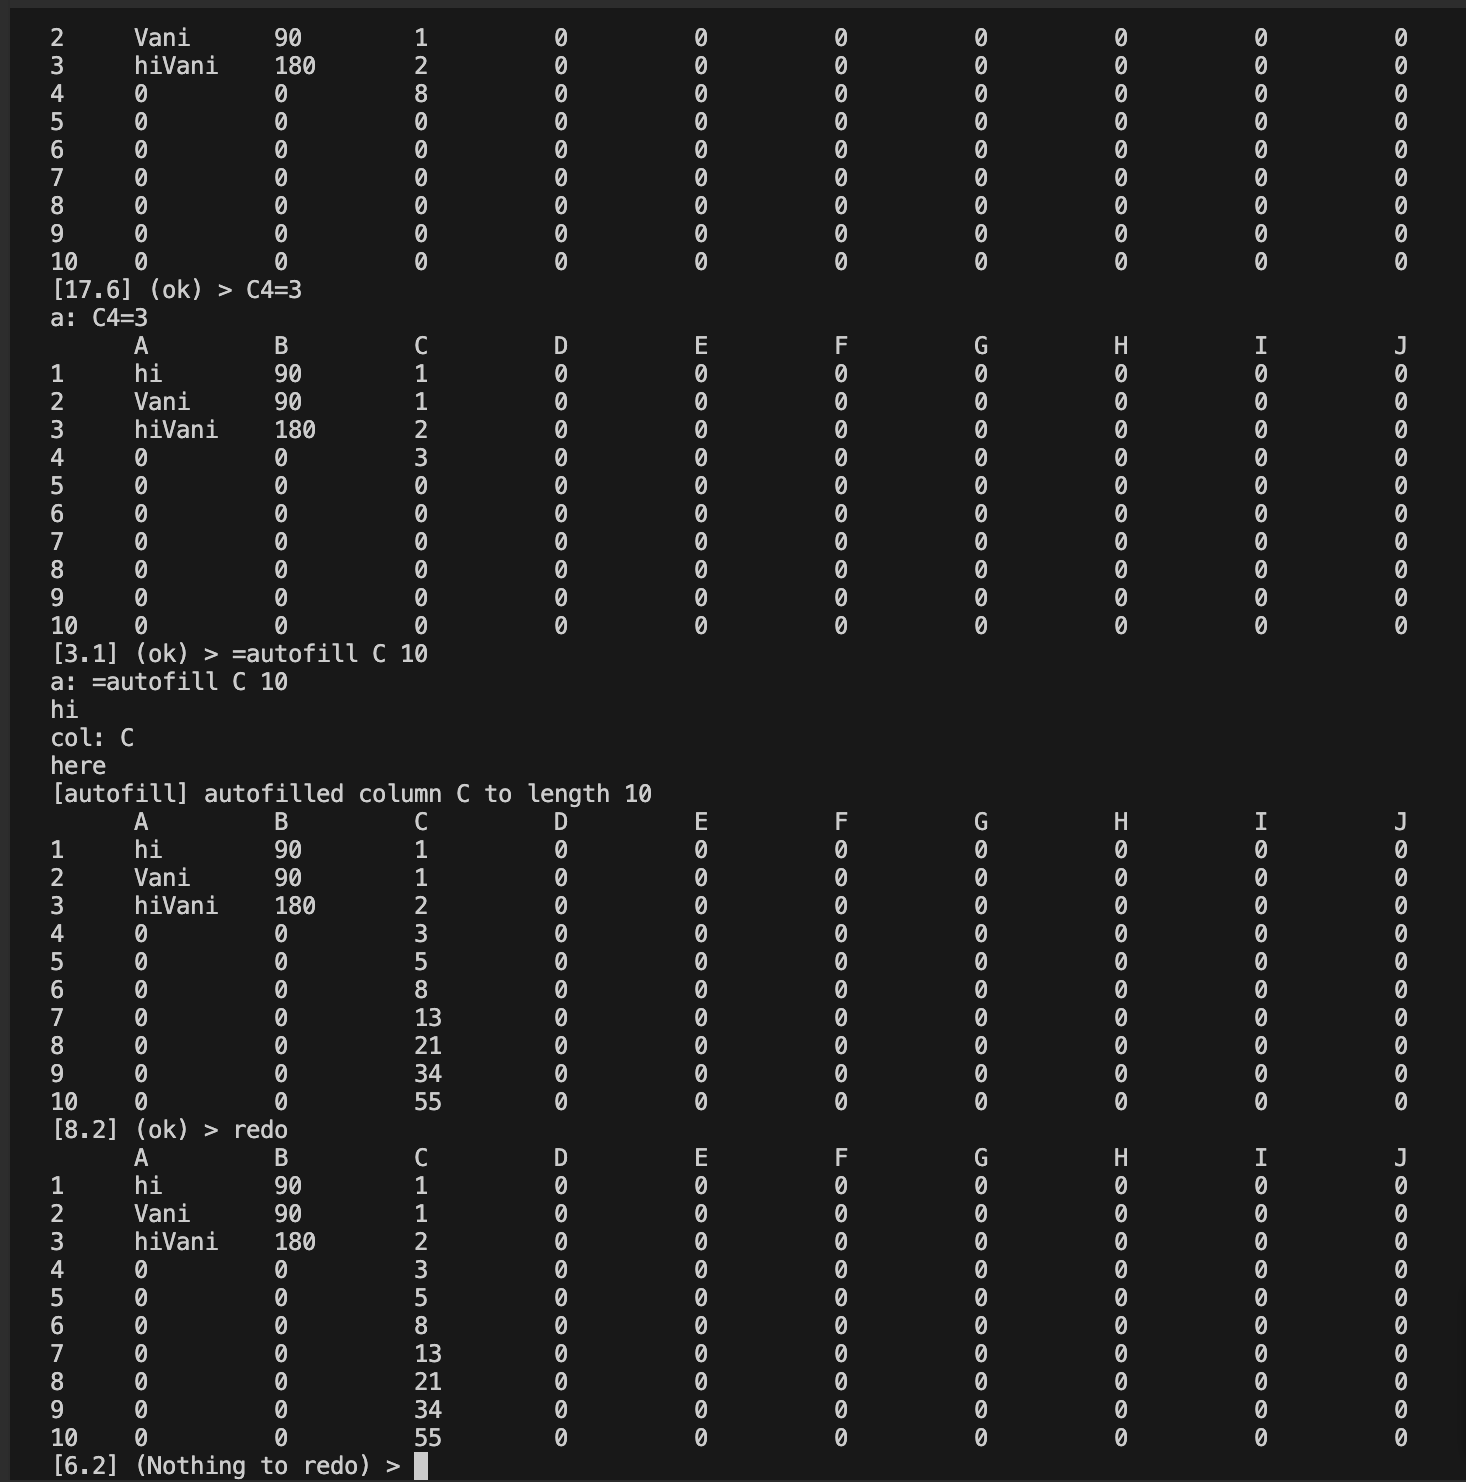
\includegraphics[width=0.5\linewidth]{image.png}
            \caption{Performing autofill for AP series, and undo}
            \label{fig:enter-label}
        \end{figure}
        
        \begin{figure}[H]
            \centering
            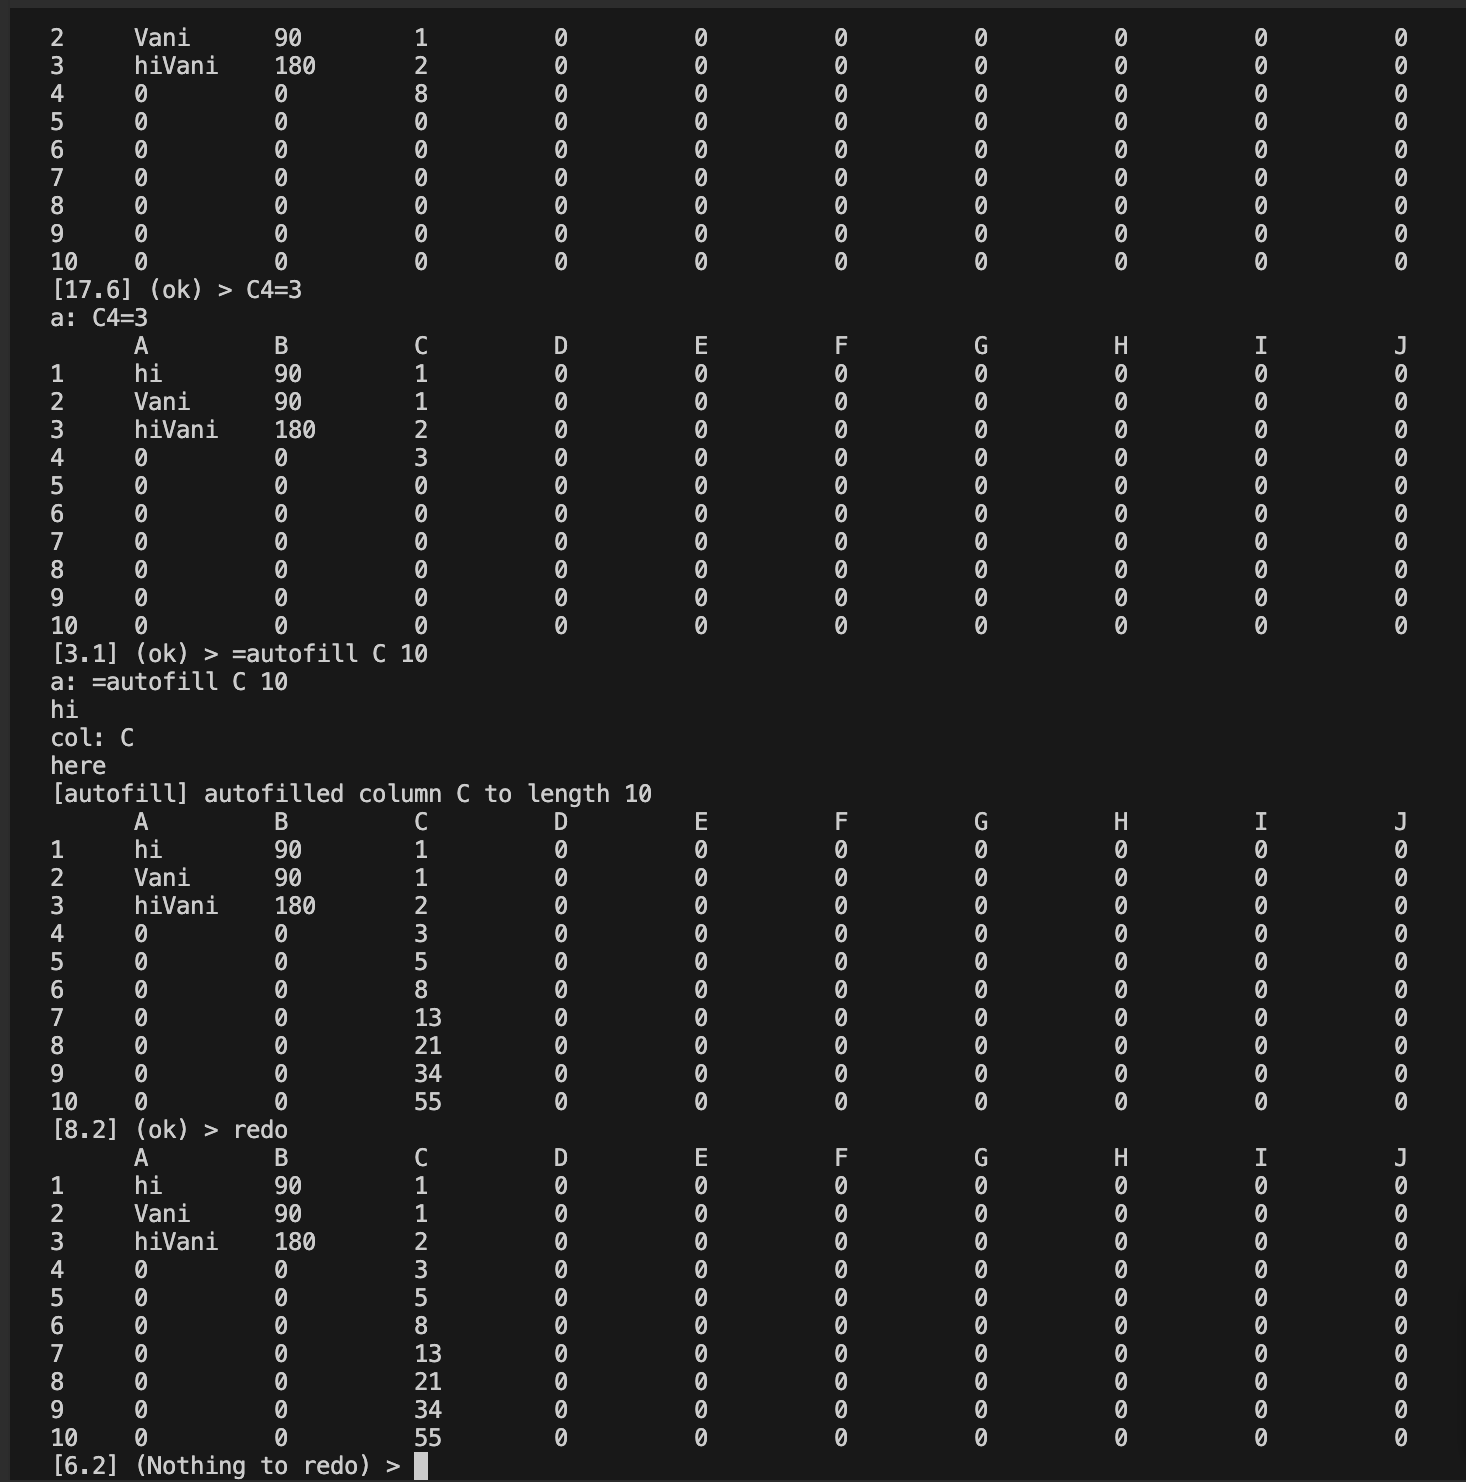
\includegraphics[width=0.5\linewidth]{image.png}
            \caption{Performing undo}
            \label{fig:enter-label}
        \end{figure}
        
        \begin{figure}[H]
            \centering
            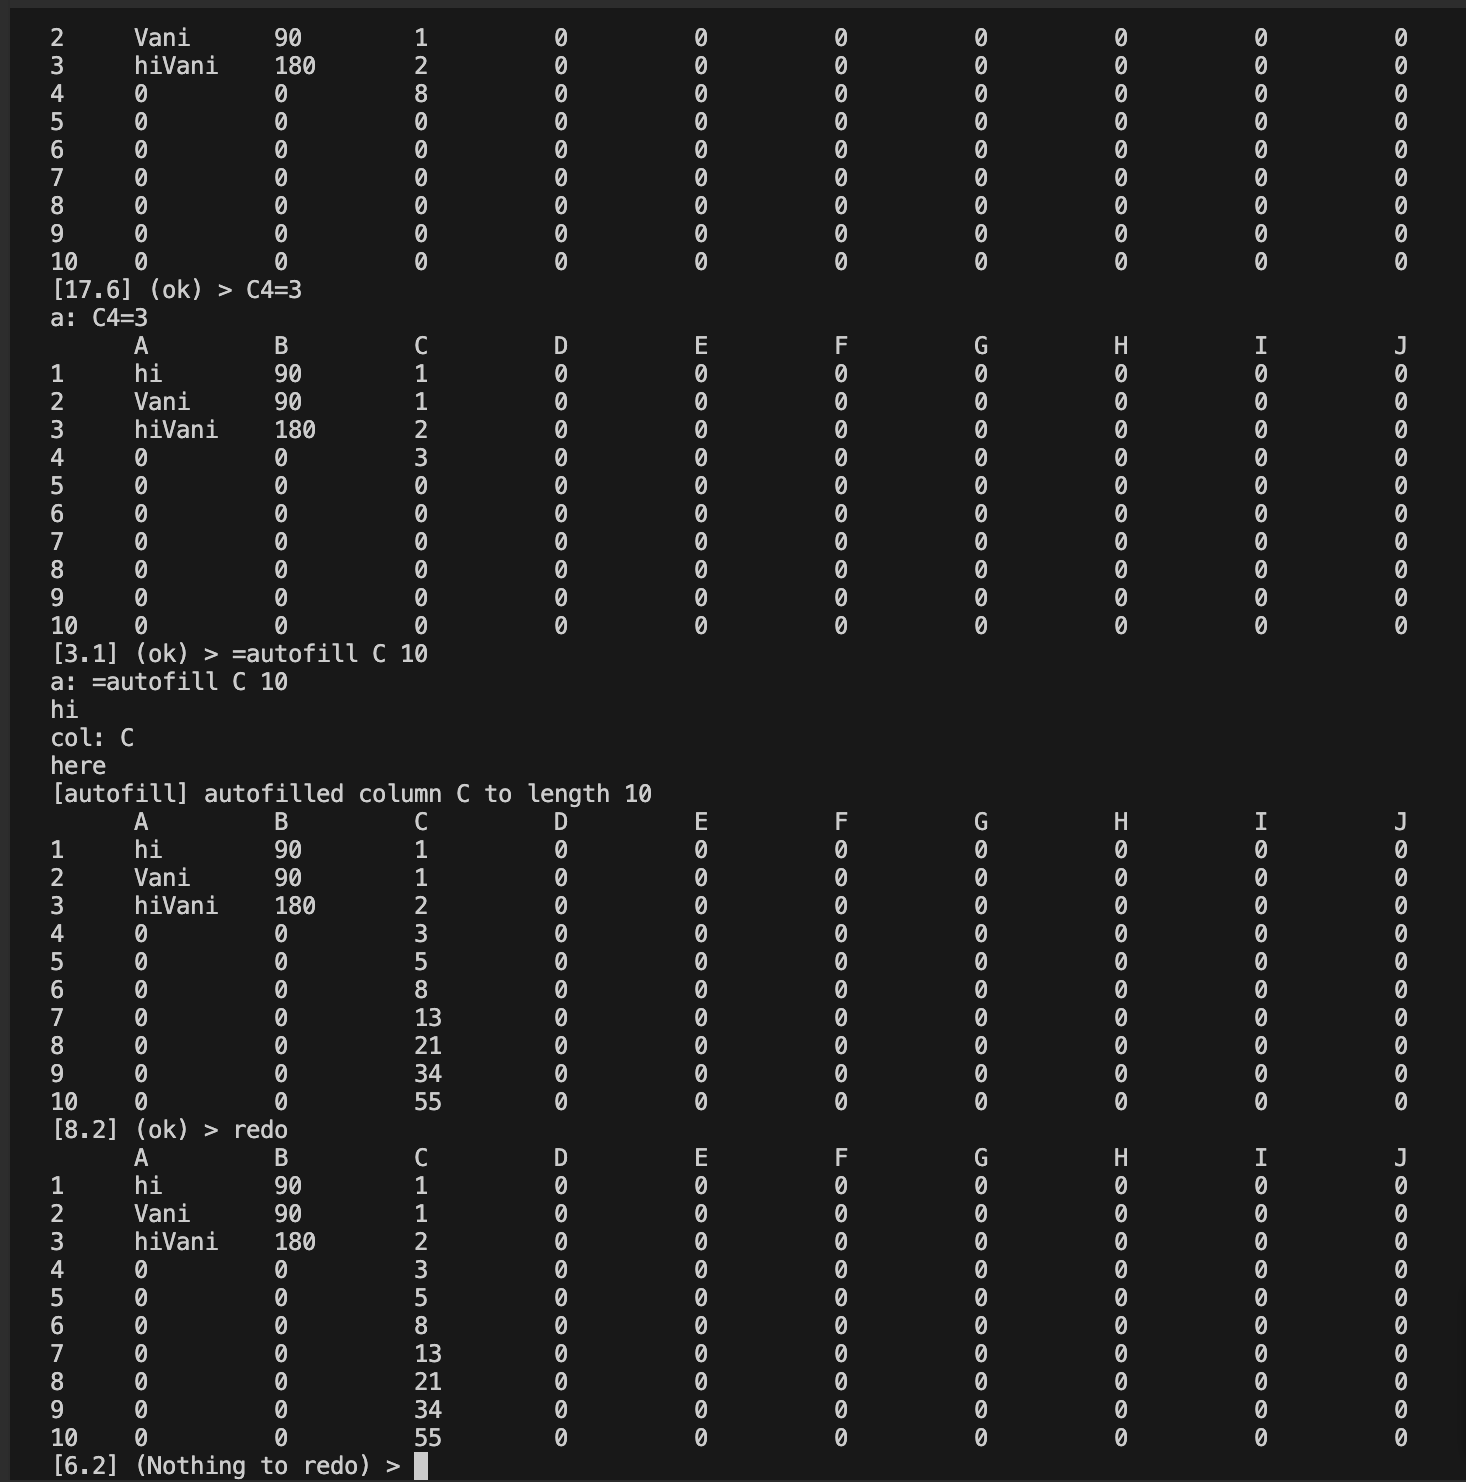
\includegraphics[width=0.5\linewidth]{image.png}
            \caption{Performing redo}
            \label{fig:enter-label}
        \end{figure}
        
        \begin{figure}[H]
            \centering
            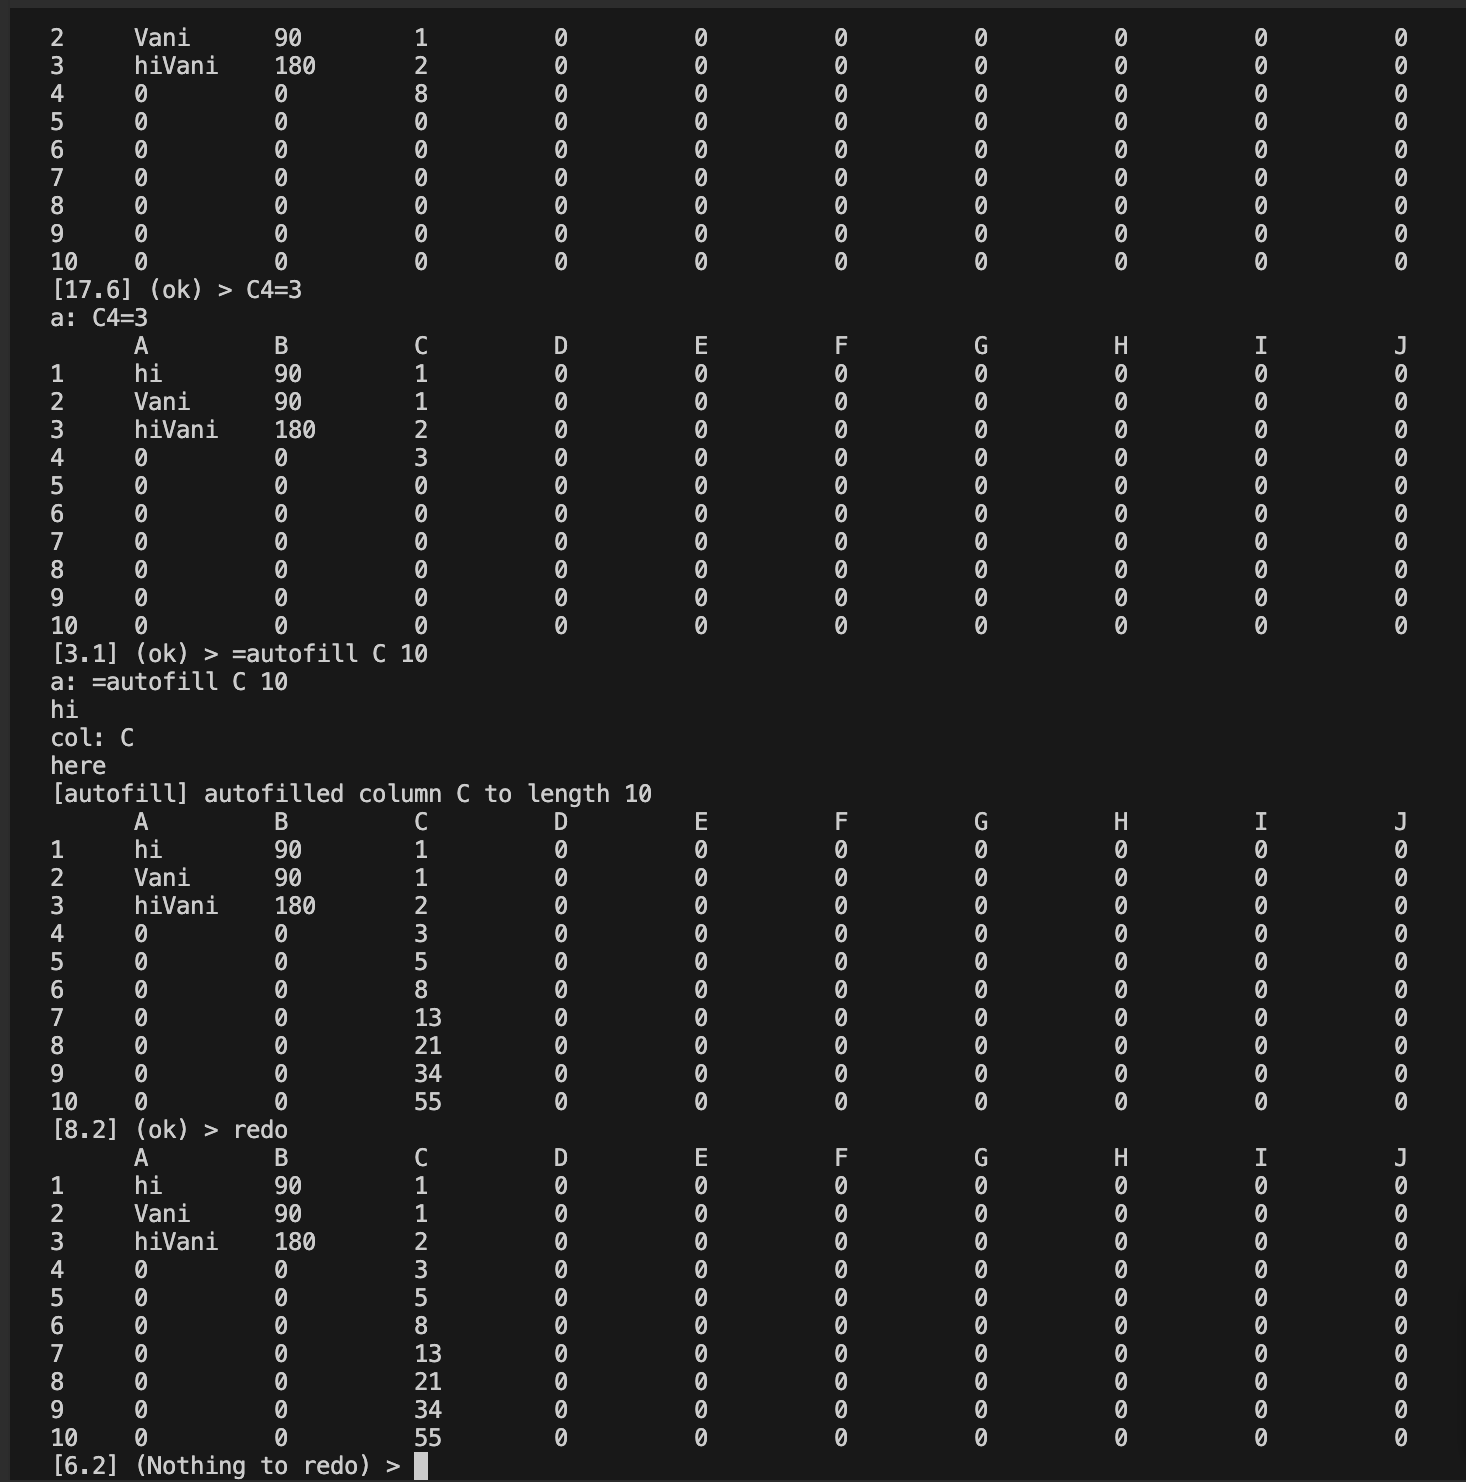
\includegraphics[width=0.5\linewidth]{image.png}
            \caption{Performing autofill for GP}
            \label{fig:enter-label}
        \end{figure}
        
        \begin{figure}[H]
            \centering
            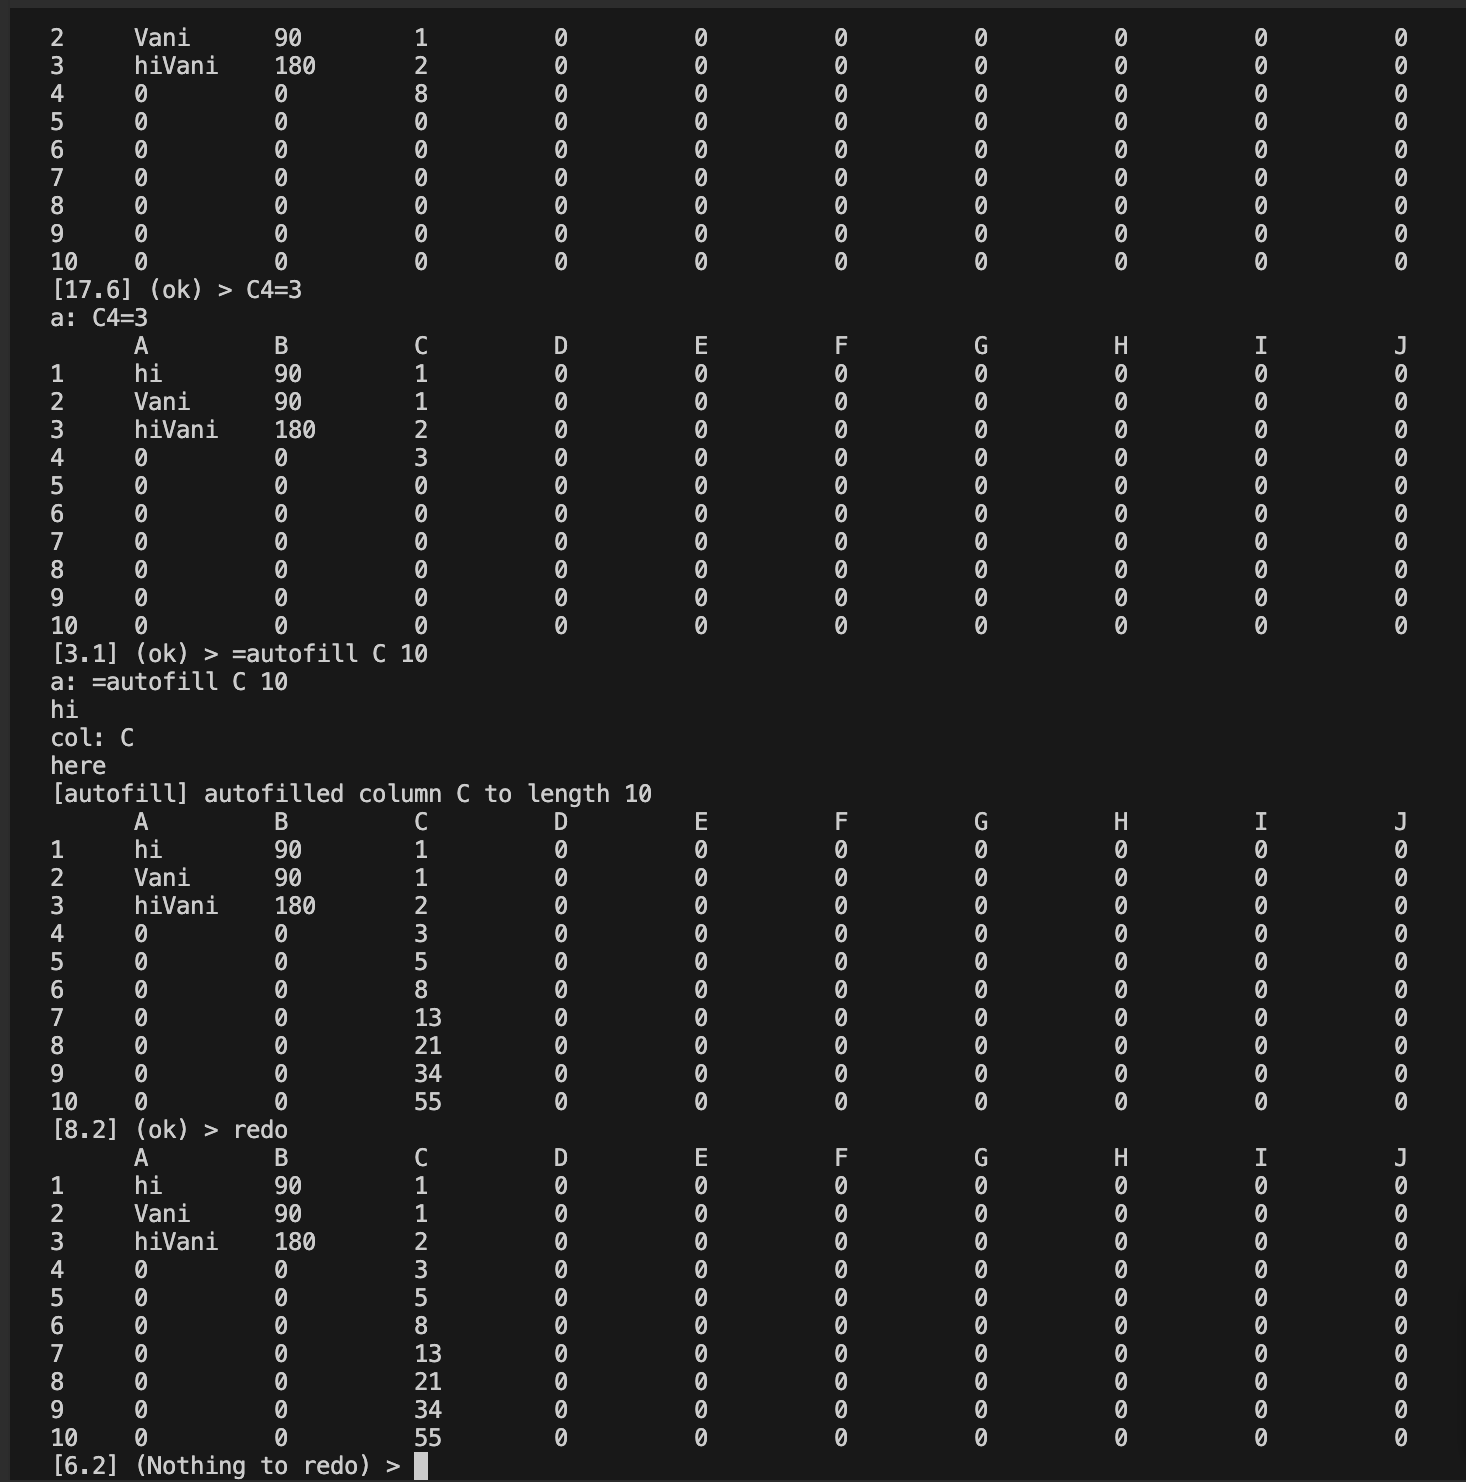
\includegraphics[width=0.5\linewidth]{image.png}
            \caption{Performing autofill for fibonacci}
            \label{fig:enter-label}
        \end{figure}
        